\section{Methodology}
This section will discuss the models used for this project. Specifically, 4 models were compared for their effectiveness with the multi fish classification problem. For the binary problem, a Res18 model was found to have excellent classification performance. 

\subsection{Res18 Architecture}
ResNet-18, as implemented in PyTorch’s torchvision, is a relatively shallow residual network designed for image classification, especially on ImageNet-sized inputs. It starts with a stem that quickly reduces spatial resolution while expanding channels. An input image of size 3×224×2243×224×224 first passes through a 7×7 convolution with 64 filters and stride 2, followed by batch normalization, a ReLU nonlinearity, and a 3×3 max-pooling layer with stride 2. After this stem, the feature map has 64 channels and a reduced resolution of 56×5656×56. This early downsampling helps keep computation manageable while extracting low-level visual features like edges and color contrasts.
\\
The core of ResNet-18 is composed of four stages of residual blocks, called BasicBlocks, stacked in sequence. Each stage maintains a fixed number of output channels but may downsample the spatial dimensions at the beginning of the stage. The first stage (layer1) uses 64 channels and contains two BasicBlocks, both with stride 1, so it preserves the 56×5656×56 resolution. The second, third, and fourth stages (layer2, layer3, layer4) have 128, 256, and 512 channels respectively, each again using two BasicBlocks. In each of those stages, the first block uses stride 2 in its first convolution (and a matching 1×1 convolution in the shortcut) to halve the spatial resolution, while the second block keeps stride 1 and uses an identity shortcut. This pattern gradually reduces the feature map from 56×5656×56 to 28×2828×28, then 14×1414×14, and finally 7×77×7, while increasing channel depth to capture more abstract features.
\\

\begin{figure}[!htpb]
\centering
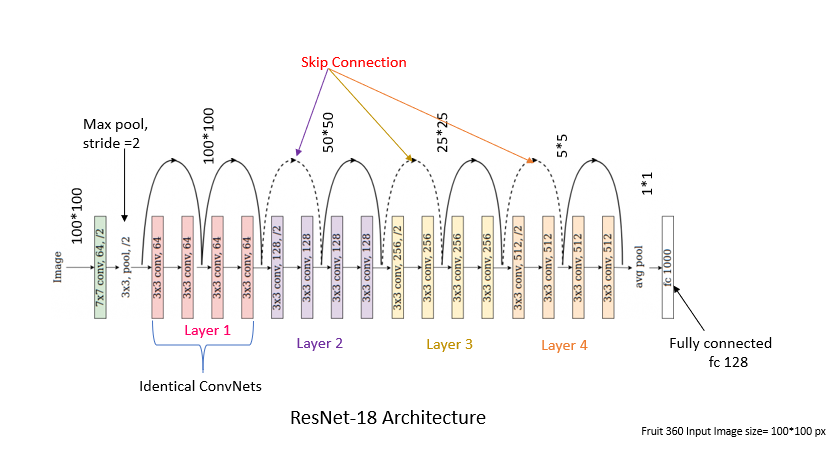
\includegraphics[width=0.8\linewidth]{./graphics/res18architecture.png}
    \caption{Architecture Description of Res18 taken from \cite{herbarium2021_half_earth_2022}}
\label{graphic:res18arch}
\end{figure}

Each BasicBlock itself has a simple but powerful structure: two 3×3 convolution layers with batch normalization and ReLU in between, plus a residual (skip) connection that adds the block’s input to its output before a final ReLU. When the input and output shapes match, the shortcut is just the identity; when the block changes resolution or channel count (for example, the first block of a new stage with stride 2), the shortcut path contains a 1×1 convolution with appropriate stride and batch normalization so that the addition is well defined. This residual design is what makes ResNet models distinctive: by learning residual functions (changes) on top of identity mappings, the network alleviates the vanishing gradient problem and allows deeper architectures to train more reliably.
\\
At the end of the four residual stages, ResNet-18 has a feature map of size 512×7×7512×7×7. Instead of using fully connected layers on flattened high-dimensional tensors, it applies a global average pooling layer that averages each of the 512 channels over the spatial dimensions, producing a compact 512-dimensional vector that summarizes the entire image. This vector then goes into a single fully connected (linear) layer mapping 512 features to the number of output classes (typically 1000 for ImageNet). The output of this final layer is a vector of logits that can be passed through a softmax for class probabilities. Overall, ResNet-18 balances depth, parameter count, and computational cost, making it a popular baseline for experiments and applications where you want the benefits of residual learning in a relatively lightweight model.

\subsection{Res50 Architecture}
ResNet-50, as commonly implemented in PyTorch’s torchvision, is a 50-layer deep convolutional neural network that builds on the residual learning idea with a more complex block called the bottleneck. The network starts with a familiar stem: an input image of size 3×224×2243×224×224 passes through a 7×7 convolution with 64 filters and stride 2, followed by batch normalization, a ReLU activation, and a 3×3 max-pooling layer with stride 2. After this stem, the feature map has 64 channels and a spatial resolution of 56×5656×56, providing a compact but expressive representation of low-level features like edges and textures. This initial stage mirrors ResNet-18/34 and prepares the data for deeper residual processing.
\\
\begin{figure}[!htpb]
\centering
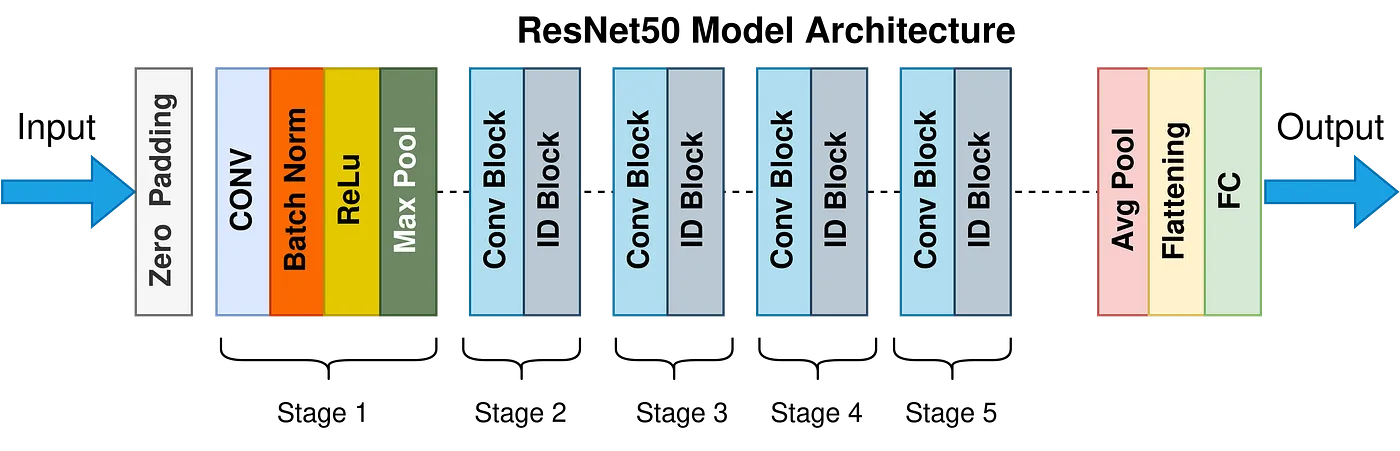
\includegraphics[width=0.8\linewidth]{./graphics/res50architecture.png}
    \caption{Architecture Description of Res50 taken from \cite{mukherjee_annotated_resnet50_2022}.}
\label{graphic:res50arch}
\end{figure}

The main body of ResNet-50 consists of four stages (often named layer1 to layer4), each made of multiple bottleneck residual blocks. Unlike the BasicBlocks used in ResNet-18, a bottleneck block uses three convolutions: a 1×1 conv that reduces the channel dimensionality, a 3×3 conv that processes features at this reduced width, and another 1×1 conv that expands back to a higher channel count (typically 4× the “base” width). In the canonical configuration for ResNet-50, these stages use 3, 4, 6, and 3 bottleneck blocks respectively, with base channel widths of 64, 128, 256, and 512. At the beginning of each new stage (except the first), the first bottleneck block uses stride 2 in its 3×3 convolution and a matching 1×1 convolution in the shortcut to downsample spatial resolution while increasing channels; the remaining blocks in that stage use stride 1 and identity shortcuts. This pattern progressively reduces the spatial size from 56×5656×56 to 28×2828×28, then 14×1414×14, and finally 7×77×7 while increasing representational depth.
\\
Each bottleneck block preserves the key residual idea: its output is the sum of the transformed input (through the 1×1–3×3–1×1 stack with batch normalization and ReLUs) and a shortcut connection that carries either the identity or a projected version of the input. The 1×1 reductions and expansions make these blocks computationally efficient, allowing the network to reach 50 layers without an explosion in parameters or FLOPs, while the skip connections help gradients flow through the deep stack during training. After the four stages, ResNet-50 has a 2048×7×72048×7×7 feature map (because of the 4× expansion in the final stage’s bottleneck blocks). A global average pooling layer then collapses each of the 2048 channels to a single value, producing a 2048-dimensional vector that summarizes the entire image. Finally, a fully connected layer maps this vector to the desired number of output classes (1000 for ImageNet), producing logits suitable for classification.

\subsection{Dense Net Architecture}
DenseNet is a convolutional neural network that connects every layer to every other layer within the same block, instead of only connecting each layer to the next one. Concretely, inside a dense block, each layer receives as input the concatenation of the feature maps produced by all previous layers, and its own output is then passed on to all subsequent layers in that block. This dense connectivity results in L(L+1)/2L(L+1)/2 direct connections for a block with LL layers, which greatly strengthens information and gradient flow through the network.
\\

\begin{figure}[!htpb]
\centering
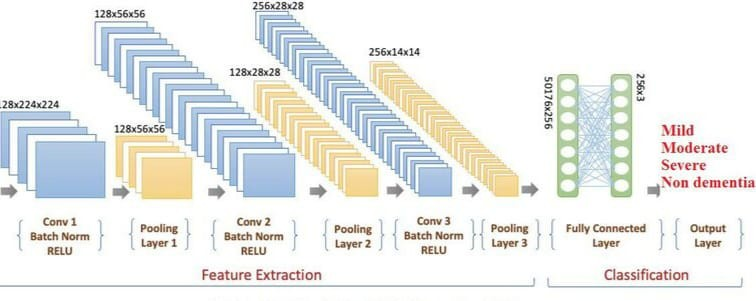
\includegraphics[width=0.8\linewidth]{./graphics/denseNetArchitecture.jpg}
    \caption{Architecture Description of DenseNet taken from \cite{favqc_densenet169_passline}.}
\label{graphic:densearch}
\end{figure}

A DenseNet is built from an initial convolutional “stem,” followed by several dense blocks separated by transition layers, and ending with global average pooling and a classifier. Dense blocks are where the dense connectivity happens; they stack multiple convolutional layers, each adding a small number of new feature maps (the growth rate) that are concatenated with all existing ones. Transition layers sit between dense blocks and use batch normalization, a 1×1 convolution, and average pooling to reduce both the number of channels and the spatial resolution, keeping the model computationally efficient as depth grows.
\\
This design has several important effects. Because each layer has direct access to the outputs of all earlier layers and to the loss signal, DenseNet largely alleviates the vanishing gradient problem and improves feature propagation. At the same time, it strongly encourages feature reuse: instead of relearning similar patterns at many depths, later layers can directly reuse earlier features, which reduces parameter redundancy and leads to compact models despite the many connections. In practice, bottleneck layers based on 1×1 convolutions are commonly used inside dense blocks to shrink the number of channels before the 3×3 convolutions, further cutting computational cost without sacrificing representational power.

\subsection{RegNet 400MF}
RegNet 400MF is a small member of the RegNet family implemented in torchvision, designed to have roughly 400 million multiply–adds at 224×224 resolution. It follows the generic RegNet template (stem → four stages of residual bottleneck blocks → global pooling and classifier), but its specific stage widths and depths are chosen by the RegNet parametrization to hit a light compute and parameter budget. Internally, torchvision computes all block widths using a linear function with parameters w0w0,
wawa (slope), wmwm (multiplicative factor), and a quantization constant, then groups consecutive blocks with identical quantized width into four stages and uses those stage widths and depths to build the network.
\\

\begin{figure}[!htpb]
\centering
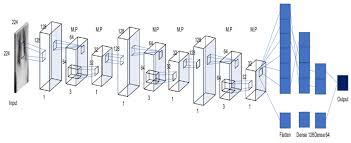
\includegraphics[width=0.8\linewidth]{./graphics/regNetArchitecture.jpg}
    \caption{Architecture Description of RegNet taken from \cite{mahub_2021}.}
\label{graphic:regarch}
\end{figure}

Architecturally, RegNetX-400MF starts with a simple convolutional stem: a 3×3 convolution with stride 2 (followed by batch normalization and nonlinearity, optionally with pooling) that reduces the input image resolution and lifts it to the initial feature width. After the stem, the network is organized into four stages operating at progressively lower spatial resolutions; each stage consists of a sequence of identical bottleneck residual blocks at a fixed width. A bottleneck block uses a 1×1 convolution to reduce channels, a 3×3 convolution (possibly grouped) to process spatial structure, and a 1×1 convolution to expand back to the stage width, with batch norm and activation layers around these convolutions and a residual skip connection from input to output. The first block in each stage handles downsampling via stride 2 in the 3×3 convolution and, if needed, a matching projection in the skip path; later blocks in the stage use stride 1 and preserve resolution.
\\
For RegNetX-400MF specifically, the RegNet parameters are chosen so that the quantized widths and resulting number of blocks per stage produce a compact model with around 4–5 million parameters and ~0.4 GFLOPs, while still following the monotonic width growth pattern characteristic of RegNet. Being an “X” variant, RegNetX-400MF does not include squeeze-and-excitation or other attention mechanisms inside the bottleneck, so its blocks are relatively simple compared to the “Y” family. This makes RegNetX-400MF a convenient lightweight backbone for experiments, resource-constrained deployments, or as a bseline architecture when exploring the RegNet design space in practice.

\subsection{Implementation Details}
Training was performed using Python 3.10 and was attempted on serveral different environments. A Dell Linux Laptop, a M1 Max Macbook Pro, and the Google Collab Lab environment. 
Ultimately, the Dell Alama Linux with a 6Gb NVIDIA A3000 graphics card was chosen as the main computer for training. This decision was made because it trained faster than the other options.
The python code was written using Vim and the project was ran from a commandline terminal.
Matplotlib was used to produce the performance plots from each model.


\begin{figure}[!htpb]
\centering
\includegraphics[width=0.8\linewidth]{./graphics/vimenv.png}
    \caption{Screenshot of Vim Environment used for coding.}
\label{graphic:vimenv}
\end{figure}


PyTorch was the machine learning library used. All of the models from TorchVision were utilized with default weights and transforms. Two sets of models were trained. A binary model to predict if a fish is present, and a multi-class model to predict a fish’s type or if there is no fish. The binary model was trained using the ResNet18 architecture and achieved a excellent performance. The multiclass problem presented a more difficult problem. 
Four models were trained and similar performancei was found between them. 

Transfer learning was utilized to improve training performance. 
It is a machine learning technique where a model that has already been trained on one task is reused as the starting point for a different but related task. Instead of learning from scratch, the model keeps its previously learned internal representations and is then fine‑tuned on the new dataset, which is often smaller. This approach reduces training time, lowers data requirements, and often improves performance, because the model builds on broadly useful features it has already discovered.

\subsection{Optimization}
This project used cross entropy for its loss function.
For a multi-class classification problem with $C$ classes, the cross-entropy
loss for a single example with one-hot label vector $\mathbf{y} \in \{0,1\}^C$
and predicted class probabilities $\hat{\mathbf{y}} \in [0,1]^C$ is
\[
\mathcal{L}_{\text{CE}}(\mathbf{y}, \hat{\mathbf{y}}) =
- \sum_{c=1}^{C} y_c \log \hat{y}_c.
\]
For a dataset of $N$ examples, we use the average cross-entropy loss
\[
\mathcal{L}_{\text{CE}} = \frac{1}{N} \sum_{i=1}^{N}
\left(
- \sum_{c=1}^{C} y_{i,c} \log \hat{y}_{i,c}
\right).
\]

The Adam optimizer was used to update the model parameters $\theta$ based on the
stochastic gradient of the loss function. Let $g_t = \nabla_{\theta} \mathcal{L}_t$
denote the gradient at step $t$. Adam maintains estimates of the first and
second moments of the gradients:
\[
m_t = \beta_1 m_{t-1} + (1 - \beta_1) g_t,
\]
\[
v_t = \beta_2 v_{t-1} + (1 - \beta_2) g_t^2,
\]
where $\beta_1, \beta_2 \in [0,1)$ are the exponential decay rates, and the
squaring is element-wise. Bias-corrected estimates are computed as
\[
\hat{m}_t = \frac{m_t}{1 - \beta_1^t}, \qquad
\hat{v}_t = \frac{v_t}{1 - \beta_2^t}.
\]
The parameter update rule for learning rate $\alpha$ and numerical stability
term $\varepsilon$ is
\[
\theta_t = \theta_{t-1} - \alpha \frac{\hat{m}_t}{\sqrt{\hat{v}_t} + \varepsilon}.
\]

\subsection{Classification Metrics}
Given the confusion matrix terms \emph{true positives} (TP), \emph{false
positives} (FP), \emph{true negatives} (TN), and \emph{false negatives} (FN),
precision, recall, F1 score, and accuracy are defined as follows.

\paragraph{Precision and Recall} For a given class,
\[
\text{Precision} = \frac{\text{TP}}{\text{TP} + \text{FP}},
\qquad
\text{Recall} = \frac{\text{TP}}{\text{TP} + \text{FN}}.
\]

\paragraph{F1 Score} The F1 score is the harmonic mean of precision and recall:
\[
\text{F1} = 2 \cdot \frac{\text{Precision} \cdot \text{Recall}}
{\text{Precision} + \text{Recall}}.
\]

\paragraph{Accuracy} Overall classification accuracy is defined as
\[
\text{Accuracy} = \frac{\text{TP} + \text{TN}}
{\text{TP} + \text{TN} + \text{FP} + \text{FN}}.
\]

In the results section, macro-averaged metrics are reported. For example precision, recall, and F1 score, are computed by first evaluating each class independently and then averaging the resulting scores across classes, giving equal weight to each class regardless of its frequency.
